

\chapter{User documentation}
\label{chap:userDoc}

In this appendix is explained how to process the \lsystems in the web user interface.
There is also a step-by-step tutorial how to create an \lsystem from scratch -- the Pythagoras tree.

\section{How to process \lsystem}

Processing of the input on the web is fairly easy.
Following explanation will be referring to \autoref{fig:processScreenExplained}.

To process the \lsystem click on the \emph{\lsystem processor} link (A) in the main menu of the web, enter the the \lsystem code into the text area (C) and click the \emph{Process \& display results} button.
Then you will see the results (D) and eventually some warnings or errors (B).

\begin{figure}[p]
	\centering
	\includegraphics[width=0.93\linewidth]{ProcessScreenExplained}
	\caption{\lsystem processing interface}
	\label{fig:processScreenExplained}
\end{figure}


\section{Creation of the Pythagoras tree}

The creation of actual \lsystem is little bit harder.
Lets start with explanation of the Pythagoras tree itself.

The Pythagoras tree is a binary tree which starts from the root\footnote{The root is at the bottom (note for computer scientists).}.
Two other branches grows each branch (including the root).
It is named by the Pythagoras because if we denote the length of the base branch as $c$ and the length of branches raised from the base branch as $a$ and $b$ the Pythagorean theorem describes theirs relation as $c^2 = a^2 + b^2$.
If the branches are drawn as squares, the formula also says that the area of the base square is equal to sum of the areas of its child squares.
The relation applies to all the squares in the tree.

Pythagoras can be easily built from squares, the angle of branches determines the size of the squares.
The branching setup is shown in \autoref{fig:pythagorasExplained}.
If we denote the left angle of the triangle as $\alpha$ and the length of the edge of the base square as $c$ then the length of the edge of the left branch is equal to the $b = c \cdot \cos(\alpha)$ and similarly for the right branch ($a = c \cdot \sin(\alpha)$).

\begin{figure}[H]
	\centering
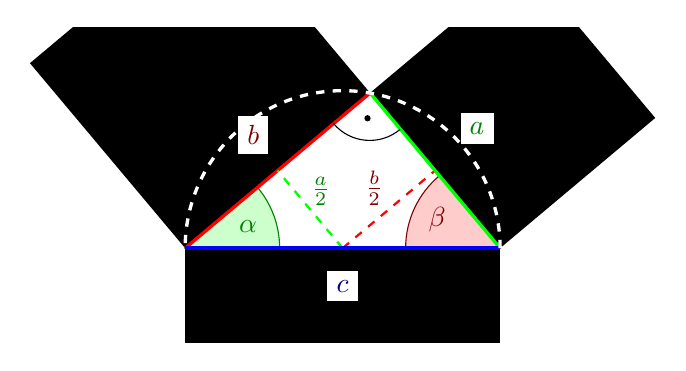
\begin{tikzpicture}[scale=4]
	\clip (-0.5,-0.3) rectangle (1.5,0.7);
	%\draw[step=.5cm,gray,very thin] (-1,-1.4) grid (2,1.4);
	
	
	\fill (0,0) rectangle (1,-1);
	\fill [rotate=40] (0,0) rectangle (0.7666,0.7666);
	\fill [xshift=1cm,yshift=0] [rotate=40] (0,0) rectangle (0.643,0.643);
	
	\draw [draw=black] (-3mm,0mm) ;
	
	\filldraw [fill=green!20,draw=green!50!black] (0,0) -- (3mm,0mm) arc (0:40:3mm) -- cycle;
	\draw [green!50!black] (0.2,0.07) node {$\alpha$};
	
	\filldraw [fill=red!20,draw=red!50!black] (1,0) -- (7mm,0mm) arc (180:130:3mm) -- cycle;
	\draw [red!50!black] (0.8,0.09) node {$\beta$};
	
	\draw [red,very thick] (0,0) -- (40:0.7666cm);
	\draw [red!50!black,very thick] (40:0.45cm) ++(130:2mm) node[below=2pt,fill=white] {$b$} (0,0);
	\draw [red,thick, dashed] (0.5,0) -- +(40:0.3833);
	\draw [red!50!black,very thick] (0.6,0.19) node {$\frac{b}{2}$};
	
	\draw [green,very thick] (40:0.7666cm) -- (1,0);
	\draw [green!50!black,very thick] (40:1cm) ++(-50:2.5mm) node[below=2pt,fill=white] {$a$} (0,0);
	\draw [green,thick, dashed] (0.5,0) -- +(130:0.3215);
	\draw [green!50!black,very thick] (0.43,0.18) node {$\frac{a}{2}$};
	
	\draw [blue,very thick] (0,0) -- (1,0);
	\draw [blue!50!black,very thick] (0.5, -0.05) node [below=2pt,fill=white] {$c$} (0,0);
	
	\draw [xshift=0.586cm,yshift=0.492cm,black,thin] (-50:1.5mm) arc (-50:-140:1.5mm);
	\fill [xshift=0.586cm,yshift=0.492cm,black] (-95:0.8mm) circle (0.1mm);
	
	\draw [draw=white,dashed,very thick] (10mm,0mm) arc (0:180:5mm);	
	
\end{tikzpicture}
	\caption{The branching in the Pythagoras tree with branches as squares}
	\label{fig:pythagorasExplained}
\end{figure}


Lets try to draw similar scheme using the \lsystem.
For drawing we will use the \emph{SvgRenderer} process configuration which renders the \lsystems with 2D turtle graphics.

Firstly, we need to draw a square.
The simplest square is a line with the same width as length.
If we look in the consolidated documentation of the \emph{SvgRenderer} process configuration (appendix \ref{chap:configurations}) in the section \emph{Interpretation methods} we can see that there is a method called \emph{DrawForward} which is exactly what we need.

Lets write our first code.
We start with the \lsystem called \emph{PythagorasTree} with the axiom containing single symbol which will be interpreted as a square.
Also we set the scale to 100 (to be able to see the result well) and initial angle to $90^{\circ}$ to start to move up (instead of right).
These properties can be found in the section \emph{Settable properties} of mentioned documentation (appendix \ref{chap:configurations}).
The code and its result is shown in \autoref{fig:userDoc1}

\newsavebox{\lstBoxUserDocA}
\begin{lrbox}{\lstBoxUserDocA}
\begin{Lsystem60}
lsystem PythagorasTree {
	set symbols axiom = S;
	set scale = 100;
	set initialAngle = 90;
	interpret S as DrawForward(1, 1);
}
process PythagorasTree with SvgRenderer;
\end{Lsystem60}
\end{lrbox}

\begin{figure}[h!]
	\subfloat{
		\usebox{\lstBoxUserDocA}
	} \hfill
	\subfloat{
		\minipage{0.37\linewidth}\noindent\centering
		\includegraphics[width=0.3\textwidth]{UserDoc1}
		\endminipage
	}
	\caption{The first square of the Pythagoras tree}
	\label{fig:userDoc1}
\end{figure}

The first problem is obvious.
By default, lines have round caps.
After a quick look into the documentation there is a property called \emph{lineCap}.
Its value 0 will remove the round caps.
To keep the source code more readable we can use a predefined constant \emph{none} for it (see appendix \ref{sec:stdLibSvgRenderer}).

\begin{Lsystem}
set lineCap = none;
\end{Lsystem}

Now we need an angle for counting the sizes of the branches.
We will define the angle as a local variable called \emph{alpha} with vale of $90^{\circ}$.
The value of the $\beta$ angle (in \autoref{fig:pythagorasExplained}) is obviously $90 - \alpha$ so we can define it as a local variable too.

\begin{Lsystem}
let alpha = 30;
let beta = 90 - alpha;
\end{Lsystem}

To be able to turn by these angles we must define an interpretation methods.
Lets define the symbol \texttt{+} as turn left by $\alpha$ degrees and symbol \texttt{-} as turn right by $\beta$ degrees (equally as turn left by $-\beta$ degrees).

\begin{Lsystem}
interpret + as TurnLeft(alpha);
interpret - as TurnLeft(-beta);
\end{Lsystem}

We need to be able to draw branches easily.
For this are the \emph{Bracketed \lsystems} which allows saving and loading of the interpretation state.
We can define the interpretation on our ow by following code.

\begin{Lsystem}
interpret [ as StartBranch;
interpret ] as EndBranch;
\end{Lsystem}

However it is much easier to just inherit the \emph{Branches} \lsystem which will do the trick.

\begin{Lsystem}
lsystem PythagorasTree extends Branches {
\end{Lsystem}

To be able to draw squares with any size we will upgrade the interpretation rule to take single parameter from the interpreting symbol and use it as line length and width.

\begin{Lsystem}
interpret S(size) as DrawForward(size, size);
\end{Lsystem}

The last thing we need to do is to skip the space between base square and the branch (mark as dotted line in \autoref{fig:pythagorasExplained}).
For this we have the interpretation method called \emph{MoveForward}.
We do not need to define explicit parameters because all parameters from interpreted symbol are automatically forwarded to the interpretation method.

\begin{Lsystem}
interpret m as MoveForward;
\end{Lsystem}


Now we can draw the squares, move without drawing, we can turn and we can do the branching so lets put it all together.
To draw a branch of the Pythagoras tree we need to
	\begin{inparaenum}[{\itshape a})]
		\item start the branch,
		\item turn left,
		\item move without drawing by half of the size of the other branch than we are drawing,
		\item draw the square and
		\item end the branch.
	\end{inparaenum}
Likewise with the right branch.

\begin{Lsystem}
set symbols axiom = S(1) // base
	 // left branch
	[ + m(1 * sin(deg2rad(alpha)) / 2) S(1 * cos(deg2rad(alpha))) ]
	 // right branch
	[ - m(1 * cos(deg2rad(alpha)) / 2) S(1 * sin(deg2rad(alpha))) ];
\end{Lsystem}

\autoref{fig:userDoc2} shows result of putting everything together along with the result.

\newsavebox{\lstBoxUserDocB}
\begin{lrbox}{\lstBoxUserDocB}
\begin{Lsystem60}
lsystem PythagorasTree extends Branches{
	let alpha = 30;
	let beta = 90 - alpha;

	set symbols axiom = S(1)
	[ + m(1 * sin(deg2rad(alpha)) / 2)
		S(1 * cos(deg2rad(alpha))) ]
	[ - m(1 * cos(deg2rad(alpha)) / 2) 
		S(1 * sin(deg2rad(alpha))) ];
	
	set scale = 100;
	set initialAngle = 90;
	set lineCap = none;
	
	interpret S(x) as DrawForward(x, x);
	interpret m as MoveForward;
	interpret + as TurnLeft(alpha);
	interpret - as TurnLeft(-beta);
}
process PythagorasTree with SvgRenderer;
\end{Lsystem60}
\end{lrbox}

\begin{figure}[h!]
	\subfloat{
		\usebox{\lstBoxUserDocB}
	} \hfill
	\subfloat{
		\minipage{0.37\linewidth}\noindent\centering
		\includegraphics[width=\textwidth]{UserDoc2}
		\endminipage
	}
	\caption{Branching of the Pythagoras thee}
	\label{fig:userDoc2}
\end{figure}

This was the hard part.
Now \lsystems will do the hard work for us.
We need to apply the creation of new branches to again and again.

Because we need to rewrite only the last level of branches we will define a new symbol \texttt{X} for already rewritten squares.
We can add it to the existing interpretation rule.

\begin{Lsystem}
interpret S X (size) as DrawForward(size, size);
\end{Lsystem}

Now for the rewrite rule.
All we need to do is to copy the axiom as the rewrite rule and use the parameter of rewritten symbol as the base size.

\begin{Lsystem}
rewrite S(x) to X(x)
	[ + m(x * sin(deg2rad(alpha)) / 2) S(x * cos(deg2rad(alpha))) ]
	[ - m(x * cos(deg2rad(alpha)) / 2) S(x * sin(deg2rad(alpha))) ];
\end{Lsystem}

To simplify the rewrite rule we can define local variables.

\begin{Lsystem}
rewrite S(x)
	with a = x * sin(deg2rad(alpha)), b = x * cos(deg2rad(alpha))
	to X(x) [ + m(a / 2) S(b) ] [ - m(b / 2) S(a) ];
\end{Lsystem}

To rewrite the \lsystem we need to set the number of iterations.
We will use lower number like 2 to see if it is working.

\begin{Lsystem}
set iterations = 2;
\end{Lsystem}

Voilà, the Pythagoras tree is growing.

\newsavebox{\lstBoxUserDocC}
\begin{lrbox}{\lstBoxUserDocC}
\begin{Lsystem60}
lsystem PythagorasTree extends Branches{
	let alpha = 30;
	let beta = 90 - alpha;

	set symbols axiom = S(1);
	
	set scale = 100;
	set initialAngle = 90;
	set lineCap = none;
	set iterations = 2;
	
	interpret S X(x) as DrawForward(x,x);
	interpret m as MoveForward;
	interpret + as TurnLeft(alpha);
	interpret - as TurnLeft(-beta);
	
	rewrite S(x)
		with a = x*sin(deg2rad(alpha)),
			b = x*cos(deg2rad(alpha))
		to X(x) [ + m(a / 2) S(b) ]
			[ - m(b / 2) S(a) ];
}
process PythagorasTree with SvgRenderer;
\end{Lsystem60}
\end{lrbox}

\begin{figure}[h!]
	\subfloat{
		\usebox{\lstBoxUserDocC}
	} \hfill
	\subfloat{
		\minipage{0.37\linewidth}\noindent\centering
		
\includegraphics[width=\textwidth]{UserDoc3}
		\endminipage
	}
	\caption{Growing Pythagoras tree}
	\label{fig:userDoc3}
\end{figure}

We can even render it into 3D with minimal effort, just process it with the \emph{ThreeJsRenderer} (and set little more iterations and green color), see \autoref{fig:UserPythagoras3D}.

\begin{Lsystem}
process PythagorasTree with ThreeJsRenderer
	set initialColor = #00AA00
	set iterations = 10;
\end{Lsystem}

\begin{figure}[p]
	\centering
	\includegraphics[width=0.7\linewidth]{UserPythagoras}
	\caption{Pythagoras tree rendered in 3D}
	\label{fig:UserPythagoras3D}
\end{figure}


If we want to generate many Pythagoras trees with different angles we can add a parameter to the \lsystem.
This parameter will be used as the $\alpha$ angle.
Then we just remove the local variable.

\begin{Lsystem}
lsystem PythagorasTree(alpha = 30) extends Branches{
\end{Lsystem}

To process more \lsystems at once with different parameters we can add more process statements.

\begin{Lsystem}
process PythagorasTree(30) with SvgRenderer;
process PythagorasTree(35) with SvgRenderer;
process PythagorasTree(40) with SvgRenderer;
process PythagorasTree(45) with SvgRenderer;
\end{Lsystem}

Final \lsystem is in \autoref{lsys:userDocFinal} and its results are in \autoref{fig:userDocFinal}

\begin{Lsystem}[label=lsys:userDocFinal,caption={Final \lsystem of the Pythagoras tree}]
lsystem PythagorasTree(alpha = 30) extends Branches{
	let beta = 90 - alpha;
	set symbols axiom = S(1);
	set scale = 100;
	set initialAngle = 90;
	set lineCap = none;
	set iterations = 10;
	interpret S X(x) as DrawForward(x,x);
	interpret m as MoveForward;
	interpret + as TurnLeft(alpha);
	interpret - as TurnLeft(-beta);
	rewrite S(x)
		with a = x*sin(deg2rad(alpha)), b = x*cos(deg2rad(alpha))
		to X(x) [ + m(a / 2) S(b) ] [ - m(b / 2) S(a) ];
}
process PythagorasTree(30) with SvgRenderer;
process PythagorasTree(35) with SvgRenderer;
process PythagorasTree(40) with SvgRenderer;
process PythagorasTree(45) with SvgRenderer;
\end{Lsystem}

\begin{figure}[p]
	\centering
	\subfloat[$\alpha = 30$]{\includegraphics[scale=0.4]{UserDocFinal30}} ~
	\subfloat[$\alpha = 35$]{\includegraphics[scale=0.4]{UserDocFinal35}}
	\\
	\subfloat[$\alpha = 40$]{\includegraphics[scale=0.4]{UserDocFinal40}} ~
	\subfloat[$\alpha = 45$]{\includegraphics[scale=0.4]{UserDocFinal45}}
	\caption{Results of finished \lsystem of the Pythagoras tree}
	\label{fig:userDocFinal}
\end{figure}






















